\usepackage{tikz}
\usetikzlibrary{positioning,shapes,shadows,arrows}

\tikzstyle{struct}=[rectangle, draw=black, text centered, anchor=north, text=black, text width=4cm]
\tikzstyle{thread}=[rectangle, draw=black, text centered, anchor=north, text=black, text width=4cm]
\tikzstyle{app}=[rectangle, draw=black, text centered, anchor=north, text=black, text width=3cm]



\newcommand{\architecture}{
\begin{figure}[h!]
\centering
    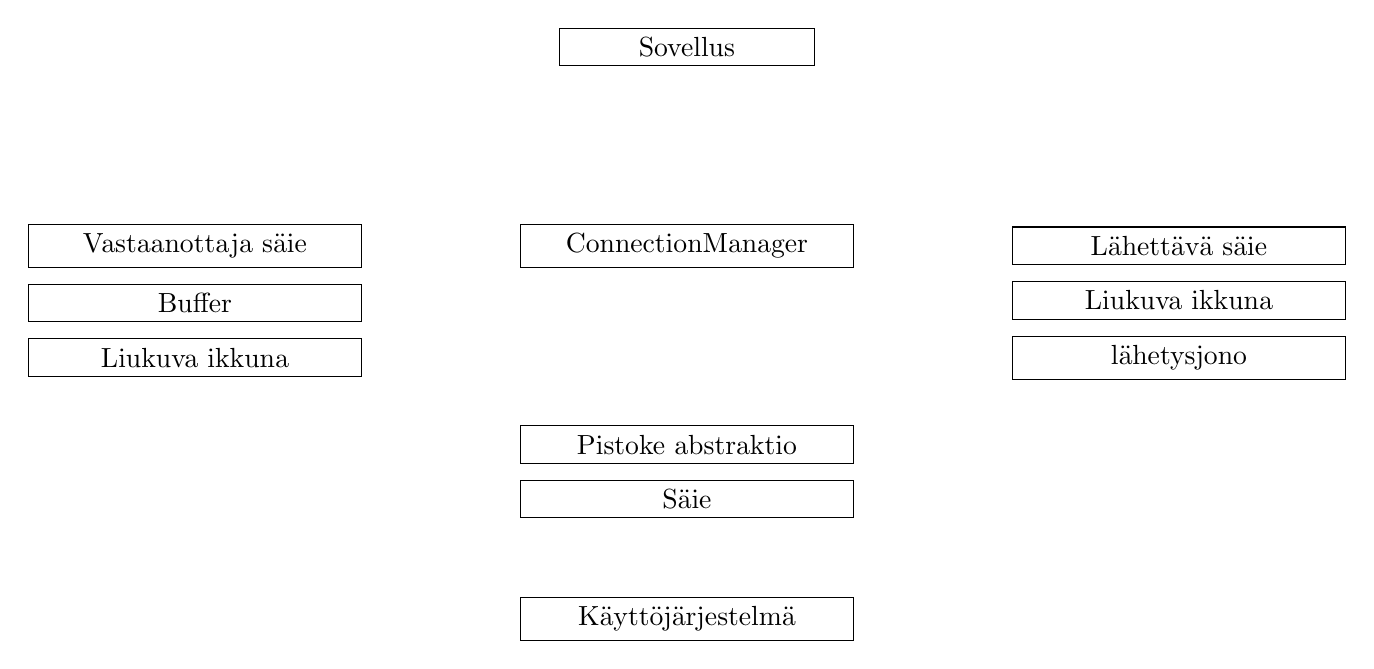
\begin{tikzpicture}[node distance=2cm]
        \node(app)[app]{
            Sovellus
        };
        \node(ConnectionManager)[struct, below=of app] {
            ConnectionManager
        };
       \node(rthread)[thread, left=of ConnectionManager]{
            Vastaanottaja säie
       };
       \node(buffer)[struct, below=0.2cm of rthread] {
            Buffer 
       };
       \node(rwindow)[struct, below=0.2cm of buffer] {
            Liukuva ikkuna 
       };
       \node(tthread)[thread, right=of ConnectionManager]{
            Lähettävä säie
       };
       \node(twindow)[struct, below=0.2cm of tthread] {
            Liukuva ikkuna 
       };
       \node(queue)[struct, below=0.2cm of twindow] {
            lähetysjono
       };
       \node(socket)[struct, below=of ConnectionManager]{
            Pistoke abstraktio
       };
       \node(socketthread)[struct, below=0.2cm of socket]{
            Säie
       };
       \node(os)[struct, below=1cm of socketthread]{
            Käyttöjärjestelmä
       };
    \end{tikzpicture}
    \caption{Arkkitehtuuridiagrammi} \label{fig:arkkitehtuuri}
\end{figure}
}